% !TeX document-id = {e3e9adc9-0b17-4199-b894-b6e314b8cf66}
% !TeX spellcheck = en_US
% !BIB program = biber 
\documentclass{article}

%% Encoding
\usepackage[T1]{fontenc}
\usepackage[utf8]{inputenc}

%% Fonts
% Math fonts (fourier) with utopia (erewhon) text fonts
\usepackage{fourier, erewhon}

%% Setup
% This package contains logos
%\usepackage[autoload]{adn}

%\setlogos[
%\textbf{Laboratório de Computação Reconfigurável}\\%[5pt]
%\uppercase{Instituto de Ciências Matemáticas e de Computação - USP}\\%[-7pt]
%]%
%{IC3D}%
%{UNICAMP}

%% Transform section references
\makeatletter
\renewcommand*{\p@section}{\S\,}
\renewcommand*{\p@subsection}{\S\,}
\makeatother

%% Shorthands
\usepackage{xspace}
\makeatletter
\DeclareRobustCommand\onedot{\futurelet\@let@token\@onedot}
\def\@onedot{\ifx\@let@token.\else.\null\fi\xspace}

\def\eg{e.g\onedot} \def\Eg{E.g\onedot}
\def\ie{i.e\onedot} \def\Ie{I.e\onedot}
\def\cf{cf\onedot} \def\Cf{Cf\onedot}
\def\etc{etc\onedot} \def\vs{vs\onedot}
\def\wrt{w.r.t\onedot} \def\dof{d.o.f\onedot}
\def\etal{et al\onedot}
\makeatother

%%%
% Other packages start here (see the examples below)
%%

%% Figues
\usepackage{graphicx}
\graphicspath{{./images-2/}}


% References
% Use this section to embed your bibliography
% Instead of having a separate file, just place the bibtex entries here
\usepackage{filecontents}% create files
\begin{filecontents}{\jobname.bib}
  @book{FP,
    title={Computer Vision A Modern Approach},
    author={David A. Forsyth, Jean Ponce},
    year={2012},
    publisher={Pearson}
  }  
  @book{SZ,
    title={Computer Vision: Algorithms and Applications},
    author={Richard Szeliski},
    year={2010},
    publisher={Springer}
  }
\end{filecontents}
% Include bibliography file
\usepackage[
backend=biber, 
style=ieee, 
natbib=true,
]{biblatex}
\addbibresource{\jobname.bib}


%% Math
\usepackage{amsmath}


%% Enumerate
\usepackage{enumitem}


\begin{document}
\title{Algoritmo Genético para Planejadores de Rotas \\
	\large Relatório de Progresso I - Agosto 2019}
\author{Gustavo de Moura Souza\thanks{Número USP 9762981, gustavo.moura.souza@usp.br}}

\maketitle

\section{Indivíduo}
\subsection{Codificação}
Seja \(t\) o tamanho do horizonte de planejamento (quantidade de waypoints que deseja-se computar), o DNA do indivíduo é definido por:
\[dna = [ gene_1, gene_2, … gene_t ] \]
\(gene_i = [ a, e ]\)para \(i = 1, … t\)
onde: \(a\) é o ângulo, e \(e\) a aceleração


\subsection{Decodificação}
seja \(x\) o conjunto de controladores do drone, para \(i = 1, … t\):

\[x = [ (px_1, py_1, v_1, al_1)_1, … (px_t, py_t, v_t, al_t)_t]\]


\(px_i\) = : Posição do VANT no eixo x
 
\(py_i\) = : Posição do VANT no eixo y

\(v_i\)  = : Velocidade do VANT na horizontal

\(al_i\) = : ângulo (direção) do VANT na horizontal



\section{Algoritmo Genético}
\subsection{Genesis - Criação da População}
Gera uma população de S indivíduos. O gene de cada indivíduo é atribuído de acordo com uma função e segue uma distribuição uniforme:
a = uniformemente distribuído entre 0.5 e 10
e = uniformemente distribuído entre 0.5 e 2*pi

\subsection{Evaluation - Computar o Valor do Fitness}
Função de fitness sendo utilizada:
fitness = f_pouso_b + f_pouso_p + f_pouso_voo_n + f_viol + f_curvas

onde:
f_pouso_b : pouso em região bonificadora
f_pouso_b(x[K], mapa) = - Cb * Somatoria( Pr(x E Z) )
Custo de pousar em região bonificadora (Cb) vezes a somatória da probabilidade de pousar em cada uma das regiões bonificadoras

f_pouso_p : pouso em região penalizadora
igual a f_pouso_p, porém substituíndo -Cb por +Cp (custo de pousar em região penalizadora)


f_pouso_voo_n : pouso ou voo sobre região não-navegável
f_pouso_voo_n = Cn * max(0 , calc)

calc = 1 - delta - Somatoria(Somatoria(Pr(x !E Z)))

Um menos delta menos somatória da somatória das probabilidades de cada um dos x não pertencer à cada uma das regiões de Zn  (loop for duplo, para cada um do controlador x a cada uma das regiões Zn), onde Zn é a região definida como não-navegável.


f_viol = realiza uma comparação de segurança
Se a aeronave tem velocidade final maior do que o seu valor mínimo, não ocorre de fato um pouso. Dessa maneira, a Equação (f_viol) evita rotas em que o VANT não consegue pousar, mesmo que atinja uma região bonificadora.

f_viol =    Cb, se vk - vminimo > 0; 
0, caso contrário

note que nesse caso o Cb está positivo, aumentando muito o valor do fitness. Lembrando que o objetivo é minizar o fitness, ou seja, quanto menor o fitness, melhor.


Pr(x E Z) e Pr(x !E Z) Probabilidade de x pertencer ou não à uma região Z:
Seja x o elemento decodificado (definido no ínicio) utiliza-se a posição cartesiana px e py para definir um ponto. Ponto este representando a posição do drone no espaço. Seja uma região composta por 4 ou mais pontos geográficos (que são convertidos para cartesiano para efeito de cálculo) definindo assim uma área.

A probabilidade é:





OBS 1: Segundo a tese do Jesimar, a função de fitness completa seria:
fitness = f_pouso_b + f_pouso_p + f_pouso_voo_n + f_curvas + f_dist + f_viol + f_bat

onde f_curvas, f_dist e f_bat eu não entendi como implementar, portanto foi definido como constante 0.




OBS 2:
Em alguns momentos é utilizado o valor K. Segundo a tese, K é o instante de tempo em que o drone sofre um acidente e entra em modo de recalcular a rota.
Como essa situação não é prevista na implementação do meu algorítimo, K é igual ao valor de t. Ou seja, a posição final do drone.
Esse valor é utilizado para os cálculos de: f_pouso_b, f_pouso_p e f_viol 












\section{Feature Descriptors}


In order to understand better feature descriptors it is important that we separate some concepts. This concepts will help us understand better the concepts we approach.

The first one we will explain is feature detectors.

\subsection{Feature Detectors}
Feature detectors are algorithms that takes patches (i.e. tiny regions) from images. This so called patches will be the base to extract relevant information in the next step. They will server as a way to know where to find the descriptor. For now, we are only talking about the detector. So the detector gets a patch from an image.

It may seem easy to take a random path, but our goal is not to make it random but instead make it relevant! If we aim to make object detection for instance, we need to assign for each object a sort of fingerprint that differentiates one object from another. This fingerprint cannot be so small and simple because we want to differentiate one from another. And they cannot be so specific that only represents a single instantiation of an object, hence it will not consider in the same category two objects of different colors for example.

With that thought, our task is to find representative patches that have this characteristics mentioned before. In image 1 we can see an explanation about the aperture problem. The aperture problem occurs when we take patches that are not so particular and due to that, can be confused by another object. Imagine we have two lines forming a corner, that is our object. We want to detect if this object matches with another in a test picture. If our patch is the corner (a) we can compare the corners and easily see that both images has corners, although, if we take a part of the line (b) or even a the low difference in gaussian (c), we may have the apperture problem.

%\begin{figure}[h]
%	\caption{Aperture problems for different image patches:  (a) stable (“corner-like”) flow;(b) classic aperture problem (barber-pole illusion); (c) textureless region. The two images I0(yellow) and I1(red) are overlaid.  The red vector u indicates the displacement between the patch centers and thew(xi)weighting function (patch window) is shown as a dark circle. (source \cite{SZ})}
%	\centering
%	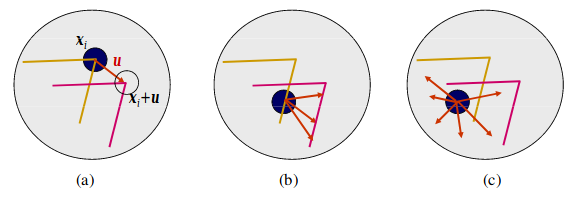
\includegraphics[width=0.8\textwidth]{apperture-problem}
% \end{figure}

\subsection{Feature Descriptors (at last)}
A feature descriptor is an algorithm that takes an image as input and, through some processing, outputs an encoded version of this image extracting relevant features about it. They encode interesting information into number (matrix, as we know).

Considering all this explanation, it is equally important that we make the descriptor to find relevant information about the image and make it specific for the task. After detecting those patches, we need to match them. We must see which one of this detections repeat in other 

\subsection{Feature Matching}
Once we have the descriptors and the relevant information encoded for some images, we can see if these descriptors match by using a set of different strategies. The most simple one is to use the least square, i.e. the squared distance between each two points. Is they are close, they probably are the same object.

There are many techniques to calculate the error and different matching strategies that impact on the efficiency of the system.



\section{SIFT}
SIFT stands for Scale Invariant Feature Transform. It as a patented algorithm for feature description. 

The SIFT features are formed by computing gradients for each small square (about 16x16 pixels) around the detected keypoint (the patch from previous explanation). Then, each keypoint receives an orientation histogram covering 360 degrees, the highest peek, i.e. the degree with most gradients pointing to, is selected and then this single vector represents the whole region as we can see on figure 2.


The SIFT algorithm is a feature descriptor, but due to this being patented, which means we cannot use without having a license, there are several other alternatives such as ORB and SURF. The feature descriptor is required for us to use on the second project, we will have to implement it. As this topic explains in a high level the SIFT algorithm, I recommend the study of the ORB algorithm, an open-source feature descriptor algorithm. It does things a little differently, but with the same objective.

As for the SIFT, after the histogram is created, it is then defined which one to use, the highest peek as mentioned. A good feature about this descriptor is that it is scale invariant, it does not varies between scales. That means that if you take a model of object with size \(X\), the algorithm will (should) detect and match the same object in different scales such as \(0.25\cdot X)\) or even \(4\cdot X\). 


\section{Finally}
This content is extend and can be broadly discussed, with this summary I intended to bring you a little about the most relevant concepts and definitions as well as the execution pipeline that relates to our second project. As I usually say, in that case write, rely on the book for further explanations and if you have trouble understanding or implementing those algorithms just ask the colleagues or the professor.

I hope my series of writing was useful and helpful, please, any suggestions let me know so I can improve and help even more.
With a warm heart, hope you enjoyed!

\printbibliography

\end{document}